% !TEX root = main.tex

\section{图像复原}
图像增强是主观的,图像复原则是客观的(恢复原图)。

空间域和频率域地退化图像分别可以由下式给出
\[\begin{aligned}
g(x,y)&=h(x,y)*f(x,y)+\eta(x,y)\\
G(u,v)&=H(u,v)F(u,v)+N(u,v)
\end{aligned}\]
关键在于怎么找回$f$和$F$,而$h$属于系统噪声。

\begin{figure}[H]
\centering
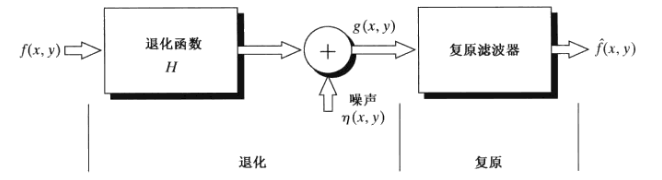
\includegraphics[width=0.8\linewidth]{fig/restoration.png}
\end{figure}

\subsection{噪声模型}
\begin{itemize}
\item 高斯噪声
\[p(z)=\frac{1}{\sqrt{2\pi}\sigma}\ee^{-\frac{(z-\bar{z})^2}{2\sigma^2}}\]
\item 脉冲/椒盐噪声
\[p(z)=\begin{cases}
P_a & z=a\\
P_b & z=b\\
1-P_a-P_b & \text{others}
\end{cases}\]
\item 瑞利噪声:均值$\bar{z}=a+\sqrt{\pi b/4}$,方差$\sigma^2=b(4-\pi)/4$
\[p(z)=\begin{cases}
\frac{2}{b}(z-a)\ee^{-(z-a)^2}{b} & z\geq a\\
0 & z<a
\end{cases}\]
\item 爱尔兰/伽马噪声:均值$\bar{z}=b/a$,方差$\sigma^2=b/a^2$
\[p(z)=\begin{cases}
\frac{a^bz^{b-1}}{(b-1)!}\ee^{-az} & z\geq a\\
0 & z<a
\end{cases},\;a>0,b\in\zz^+\]
\item 指数噪声:均值$\bar{z}=1/a$,方差$\sigma^2=1/a^2$
\[p(z)=\begin{cases}
a\ee^{-az} & z\geq 0\\
0 & z<0
\end{cases}\]
\item 均匀噪声:均值$\bar{z}=(a+b)/2$,方差$\sigma^2=(b-a)^2/12$
\[p(z)=\begin{cases}
\frac{1}{b-a} & a\leq z\leq b\\
0 & \text{others}
\end{cases}\]
\end{itemize}
\begin{figure}[H]
\centering
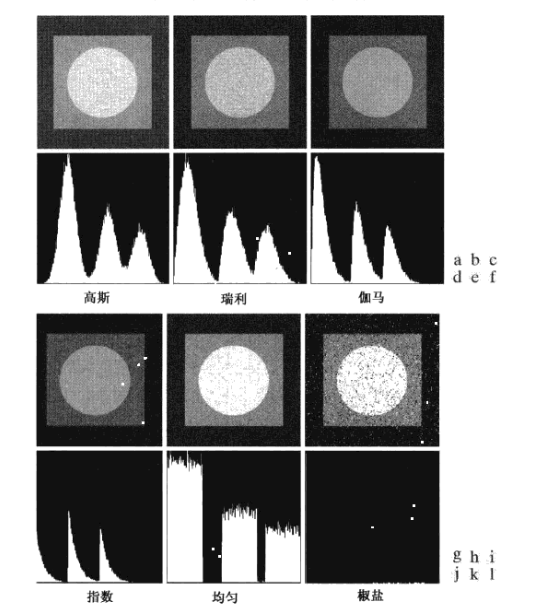
\includegraphics[width=0.5\linewidth]{fig/noise.png}
\end{figure}

\subsection{噪声存在下的空间滤波复原}
考虑唯一存在噪声退化,即不存在系统退化,则原式变为
\[\begin{aligned}
g(x,y)&=f(x,y)+\eta(x,y)\\
G(u,v)&=F(u,v)+N(u,v)
\end{aligned}\]

\subsubsection{均值滤波器}
\begin{itemize}
	\item 算术均值滤波
	\[\hat{f}(x,y)=\frac{1}{MN}\sum_{(s,t)\in S_{xy}}g(s,t)\]
	\item 几何均值滤波
	\[\hat{f}(x,y)=\lrs{\prod_{(s,t)\in S_{xy}}g(s,t)}^{\frac{1}{mn}}\]
	相比算术均值,丢失图像细节比较少
	\item 谐波均值滤波
	\[\hat{f}(x,y)=\frac{mn}{\sum_{(s,t)\in S_{xy}}\frac{1}{g(s,t)}}\]
	对盐(大的)噪声比较好,对胡椒噪声不好,善于处理高斯噪声
	\item 逆谐波均值滤波
	\[\hat{f}(x,y)=\frac{\sum_{(s,t)\in S_{xy}}g(s,t)^{Q+1}}{\sum_{(s,t)\in S_{xy}}g(s,t)^Q}\]
	其中$Q$称为滤波器的阶数,适合减少椒盐噪声的影响。
	当$Q$为正时,消除胡椒噪声;当$Q$为负时,消除盐粒噪声;但不能同时消除这两种噪声。
	当$Q=0$时退化为算术均值,$Q=-1$为谐波均值滤波
\end{itemize}